\documentclass[a4paper, 11pt]{article}

\usepackage[francais]{babel}
\usepackage[utf8]{inputenc}
\usepackage[T1]{fontenc}

\usepackage{float}
\usepackage{graphicx}
\usepackage{comment} % enables the use of multi-line comments (\ifx \fi)
\usepackage{fullpage} % changes the margin
\usepackage{multirow}

\setlength{\parindent}{0pt}
\setlength{\parskip}{0.5em plus0.3em minus0.2em}

\begin{document}

\large\textbf{\'Etude Technologique 1} \hfill \textbf{Distribution de l'eau en Haïti} \\
\normalsize Deknop Céline \hfill Université Catholique de Louvain \\
Hallet Adrien \hfill \today \\
Strebelle Sébastien

\section*{Abstract}
\'Ce document companion a été produit lors de l'évaluation de plusieurs frameworks disponibles pour une application web.
%Todo : peut-être update l'abstract une fois fini

\hrule
\section*{Frameworks}
\textit{Liste non-exhaustive et partiellement subjective basée sur les données exposées ci-dessous}.

\begin{table}[H]
    \centering
    \begin{tabular}{|c|c||c|c|c|c|c||c|}
        \hline
        \textbf{Langage} & \textbf{Framework} & \textbf{C} & \textbf{M} & \textbf{Pe} & \textbf{Po} & \textbf{T} & \textbf{Total} \\
        \hline
        \multirow{4}{*}{\textbf{JavaScript}} & Angular & M & M & B & B & M &3.5 \\
         & MeteorJS & B & B & M & N & B & 3.5\\
         & NodeJS & M & M & M & B & N & 3.5\\
         & React & B & B & M & B & B & 4.5\\
        \hline
        \multirow{3}{*}{\textbf{Python}} & Django & M & M & B & B & M& 3.5\\
         & Flask & B & B & B & B & B & 5\\
         & Pyramid & B & B & B & N & B & 4\\
        \hline
        \multirow{1}{*}{\textbf{Ruby}} & Rails & N & M & B & B & B & 3 \\
        \hline
    \end{tabular}
\end{table}
\subsection*{Critères - [B]on, [M]oyen, [N]égatif}
\begin{description}
    \item[C] Complexité - Difficulté d'utilisation / apprentissage
    \item[M] Maintenabilité - Aisance et possibilités de maintenance
    \item[Pe] Performance - Capacités du framework en termes de vitesse
    \item[Po] Popularité - Popularité du langage à travers le monde
    \item[T] Taille - Espace de stockage requis
\end{description}

\section*{C - Complexité}
\'Evaluer la complexité est hautement subjective en fonction des préférences et habitudes du développeur. Nous pouvons néanmoins comparer les langages utilisés et la structure du framework.

Une mesure de la complexité se base sur l'imbrication des blocs de code. Un code comportant beaucoup de structures imbriquées sera moins lisible, et donc plus complexe. Les résultats\footnote{\'Etude de Seerene\copyright, 2015} en figure~\ref{fig:complexity} montrent que cette mesure favorise le langage Python.

\begin{figure}
    \centering
    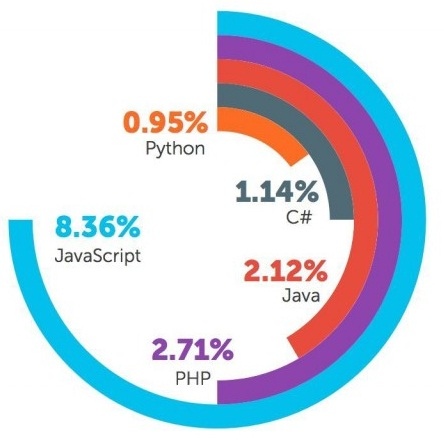
\includegraphics[width=.6\textwidth]{Etude_Technologique_1/complexity}
    \caption{Pourcentage de code imbriqué}
    \label{fig:complexity}
\end{figure}

La figure~\ref{fig:sloc_comparison} représente un comparatif\footnote{http://blog.wolfram.com/2012/11/14/code-length-measured-in-14-languages/} effectué par Wolfram\copyright (plateforme mathématique bien connue) mesurant la quantité de lignes de code nécessaires dans un langage pour reproduire un programme donné dans un autre langage. Le nombre de lignes de code n'est toutefois que partiellement une mesure de la complexité car toute ligne de code ne s'équivaut pas en terme de complexité.

\begin{figure}
    \centering
    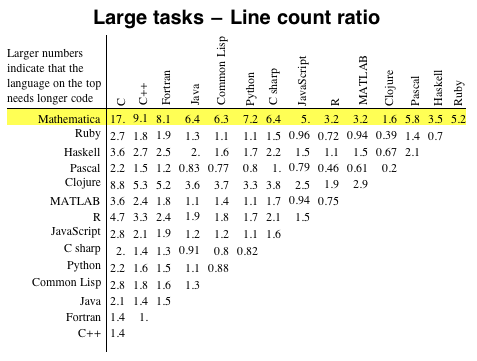
\includegraphics[width=.8\textwidth]{Etude_Technologique_1/sloc_comparison.png}
    \caption{Nombre de lignes de code nécessaires pour traduire un programme}
    \label{fig:sloc_comparison}
\end{figure}

\section*{M - Maintenabilité}
L'aisance avec laquelle un code est maintenu à jour est inversement lié à la complexité. A cela, nous pouvons ajouter les fréquences de mise à jour des frameworks. La structure du framework impacte également la maintenabilité ; moins on modifie de fichiers pour implémenter une fonctionnalité, mieux c'est.

\section*{Pe - Performance}
Bien que moins importantes que dans une application critique (e.g.: aérospatial), les performances sont mesurées en termes de temps de réponse.

\section*{Po - Popularité}
La popularité est sans doute la plus importante des mesures de ce comparatif. Un langage populaire dispose de plus de tutoriels et aide en ligne que d'obscurs langages / frameworks peu ou pas utilisés.

La figure~\ref{fig:hotframework} montre une évolution\footnote{https://hotframeworks.com/} de la popularité des frameworks les plus courants.

\begin{figure}
    \centering
    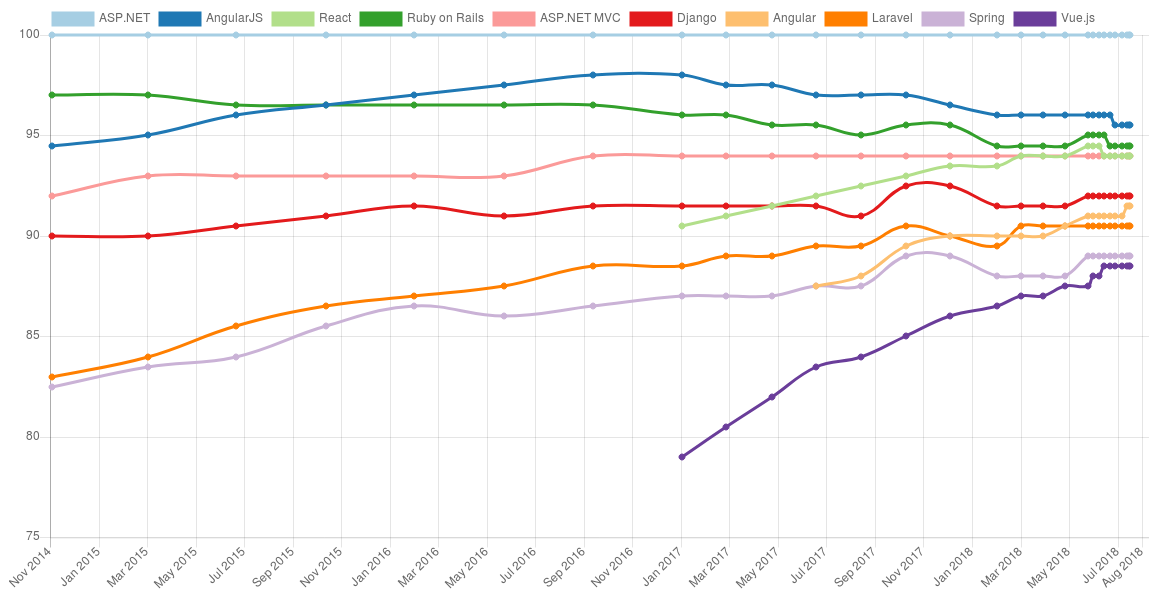
\includegraphics[width=\textwidth]{Etude_Technologique_1/hotframework.png}
    \caption{Popularité des frameworks de novembre 2014 à aujourd'hui}
    \label{fig:hotframework}
\end{figure}

\section*{T - Taille}
Un framework léger sera plus intéressant pour ce projet. D'une part pour la complexité, car moins il est nécessaire de modifier/ajouter des fichier, plus l'utilisation est aisée. D'autre part car le serveur de destination nous est inconnu et nous ne savons donc pas quel espace de stockage sera mis à disposition.

\section*{Critères spéciaux}

Notons qu'en lien avec un autre projet, il serait utile d'employer le système de géo-représentation GeoNode. \textbf{GeoNode est orienté Django} et ne peut pas être utilisé avec d'autres frameworks.

\textit{D'autres critères spéciaux pourront se rajouter avec la réunion du 03 septembre 2018.}

\section*{Autres}

La taille de l'application sera peu dépendante du framework utilisé en back-end. La majeure partie du poids du site (hormis les données) sera attribuée au front-end et donc dépendante du système front-end utilisé

\section*{Conclusion}

Le choix d'un framework repose au final sur de nombreux critères dont plusieurs sont subjectifs. L'expérience est bien souvent facteur décisif.

Il existe de très nombreux frameworks et la liste ci-dessus ne saurait être exhaustive. Les frameworks lourds, peu performants ou inadaptés à la construction de l'application décrite n'ont pas été explorés (Java, PHP, ...).

Au final, le choix se limitera surtout entre les frameworks JavaScript et Python en raison de leur très grande popularité dans les applications web pour petites entreprises. Les framework Python se démarquent positivement et si Flask semble être le meilleur choix pour notre projet, Django n'en reste pas moins un second choix de qualité qui pourrait être choisi en raison du module \textbf{GeoNode}.

\end{document}
